\documentclass{beamer}

\title{Introduction to AI and ML}
\subtitle{Matrix Project}
\author{Binaya Kumar Sahoo(EE17BTECH11048),
		\\Hrithik Pawar(EE17BTECH11006)}

%\usetheme{lucid}
\begin{document}
	\frame {
		\titlepage
	}
	\frame {
		\frametitle{Geometry Question:}
		The point
		\[\begin{pmatrix}
		2\\1
		\end{pmatrix}\]
		is translated parallel to the line
		\begin{equation}
		\begin{pmatrix}
		1&-1\\
		\end{pmatrix}\bold{x}=4
		\end{equation}
		by $2\sqrt{3}$ units. If the new point $\bold{B}$ lies in the third quadrant, then find the equation of the line 				passing through $\bold{B}$ and perpendicular to $L$.
			}
	\frame{
		\frametitle{Approach to Question:}
		The required point which is at a distance of $2\sqrt{3}$ units can be found by adding the given point with 					$2\sqrt{3}$ times the direction vector of the given line. Then the equation of the required line is calculated by 				using slope of given line.
	}
	\frame{
	    \frametitle{Solution in Matrix form:}
	    Given point:
	    \begin{equation}
	    \bold{A}=\begin{pmatrix}
		2\\1
		\end{pmatrix}
		\end{equation}
		Given line:
		\begin{equation}
		L_1:\begin{pmatrix}
		1&-1\\
		\end{pmatrix}\bold{x}=4
		\end{equation}
		Normal vector of given line:
		\begin{equation}
	    \bold{n}_1=\begin{pmatrix}
		1\\-1
		\end{pmatrix}
		\end{equation}
		Direction vector of given line:
		\begin{equation}
	    \bold{m}_1=\begin{pmatrix}
	    0&1\\
	    -1&0
	    \end{pmatrix}
	    \bold{n}_1=
	    \begin{pmatrix}
	    0&1\\
	    -1&0
	    \end{pmatrix}
	    \begin{pmatrix}
		1\\-1
		\end{pmatrix}=
		\begin{pmatrix}
		-1\\-1
		\end{pmatrix}
		\end{equation}
		
	}
	\frame{
		\frametitle{Solution in Matrix form:(contd)}
		Required point:
		\begin{equation}
	    \bold{B}=\bold{A} + 2\sqrt{3}*\bold{m}_1/\sqrt{2}
		\end{equation}
		or
		\begin{equation}
	    \bold{B}=\begin{pmatrix}
		2\\1
		\end{pmatrix} + 2\sqrt{3}*\begin{pmatrix}
		-1\\-1
		\end{pmatrix}/\sqrt{2}
		\end{equation}
		or
		\begin{equation}
	    \bold{B}=\begin{pmatrix}
		2-\sqrt{6}\\1-\sqrt{6}
		\end{pmatrix}
		\end{equation}		
	}
	\frame{
		\frametitle{Solution in Matrix form:(contd)}
		Slope of reqd. line:
		\begin{equation}
	    \bold{m}_2=\bold{n}_1=\begin{pmatrix}
		1\\-1
		\end{pmatrix}
		\end{equation}
		Normal vector of reqd. line:
		\begin{equation}
	    \bold{n}_2=\bold{m}_1=\begin{pmatrix}
		-1\\-1
		\end{pmatrix}
		\end{equation}
		Therefore, equation of reqd. line:
		\begin{equation}
	    L_2:\bold{n}_2^T(\bold{x}-\bold{B})=0
		\end{equation}
		or
		\begin{equation}
	    \begin{pmatrix}
		-1&-1\\
		\end{pmatrix}
		\bold{x}=-\begin{pmatrix}
		-1&-1\\
		\end{pmatrix}
		\begin{pmatrix}
		2-\sqrt{6}\\1-\sqrt{6}
		\end{pmatrix}
		\end{equation}
		or
		\begin{equation}
	    L_2:\begin{pmatrix}
		-1&-1\\
		\end{pmatrix}
		\bold{x}=3-2\sqrt{6}
		\end{equation}
	}
	\frame{
		\frametitle{Solution Figure:}
		\begin{figure}
    		\centering
    		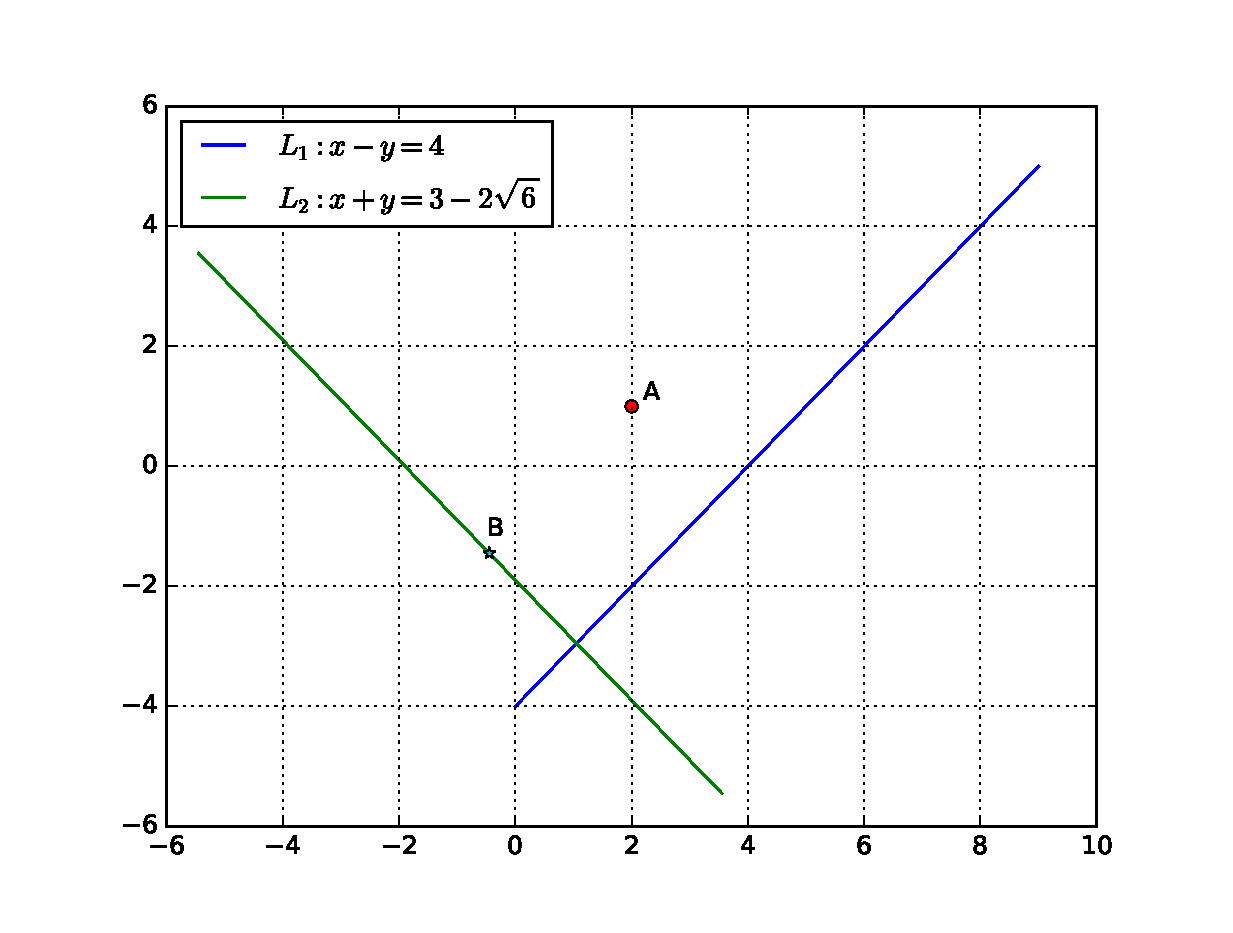
\includegraphics[width = 0.9\textwidth]{./figure.eps}
  		\end{figure}
	}	
\end{document}